%\documentclass[9pt,journal,draftcls,letterpaper,twocolumn]{article}
\documentclass[conference]{IEEEtran}

%\usepackage{graphicx}
\usepackage{amsmath,amssymb}    % need for subequations
\usepackage[dvips]{graphicx}   % need for figures
\usepackage{verbatim}   % useful for program listings
\usepackage{color}      % use if color is used in text
\usepackage{subfigure}  % use for side-by-side figures
\usepackage{hyperref}   % use for hypertext links, including those to external documents and URLs
\usepackage{epsfig}
\usepackage{float}


\begin{comment}
\pagestyle{empty} % use if page numbers not wanted
\end{comment}
\DeclareMathOperator*{\argmin}{arg\,min}

% above is the preamble

\begin{document}


\begin{figure} [H]
\centering
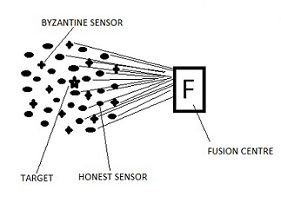
\includegraphics{MODEL.png}
\caption{Sensor Model }
\label{F1}
\end{figure}
\begin{figure} [H]
\centering
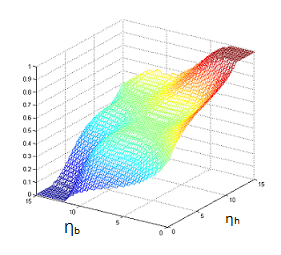
\includegraphics{alpha_blind.png}
\caption{Plot of $\alpha_{blind}$ versus honest and byzantine sensor's threshold $\eta_h$ and $eta_b$ }
\label{F2}
\end{figure}

\begin{figure} [H]
\centering
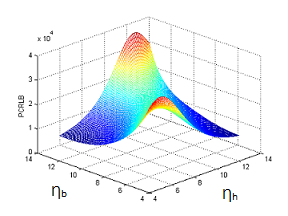
\includegraphics{mesh_pcrlb_trace.png}
\caption{Plot of tr(PCRLB) versus honest and byzantine sensor's threshold, $\eta_h$ and $eta_b$, we can see that saddle point exist }
\label{F3}

\end{figure}
\begin{figure} [H]
\centering
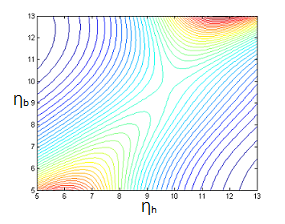
\includegraphics{contour_pcrlb_trace.png}
\caption{Plot of contour of the surface of tr(PCRLB)shown in Fig. 2.}
\label{F4}
\end{figure}

\begin{figure} [H]
\centering
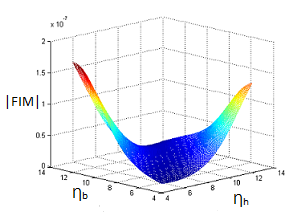
\includegraphics{mesh_det_fim.png}
\caption{Plot of $|FIM|$ versus honest and byzantine sensor's threshold, $\eta_h$ and $eta_b$, we can see that saddle point exist}
\label{F5}
\end{figure}

\begin{figure} [H]
\centering
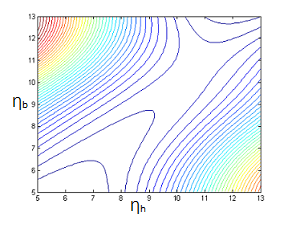
\includegraphics{contour_det_fim1.png}
\caption{Plot of contour of the surface of $|FIM|$ shown in Fig. 4.}
\label{F6}
\end{figure}


\end{document}




